% Image fixe de l'animation rsjs-niveaux. Lignes de niveau de l'erreur dans le plan
% (alpha - alpha*, beta - beta*), gamma choisi au mieux : q(d) = d^T B d.
% Nuage : quatre points en u = -1, quatre en v = 1,5, un point en c.
% c = 0,25 : B = [[5,295 ; 6,25] ; [6,25 ; 12,5]], valeurs propres 1,684 et 16,11,
%   vecteur propre de la petite à -30,02 degrés : ellipses.
% c = u = -1 : valeurs propres 0 et 17,36, noyau dirigé par (1, -(u+v)) = (1, -0,5) :
%   droites parallèles, droite orange des minimiseurs.
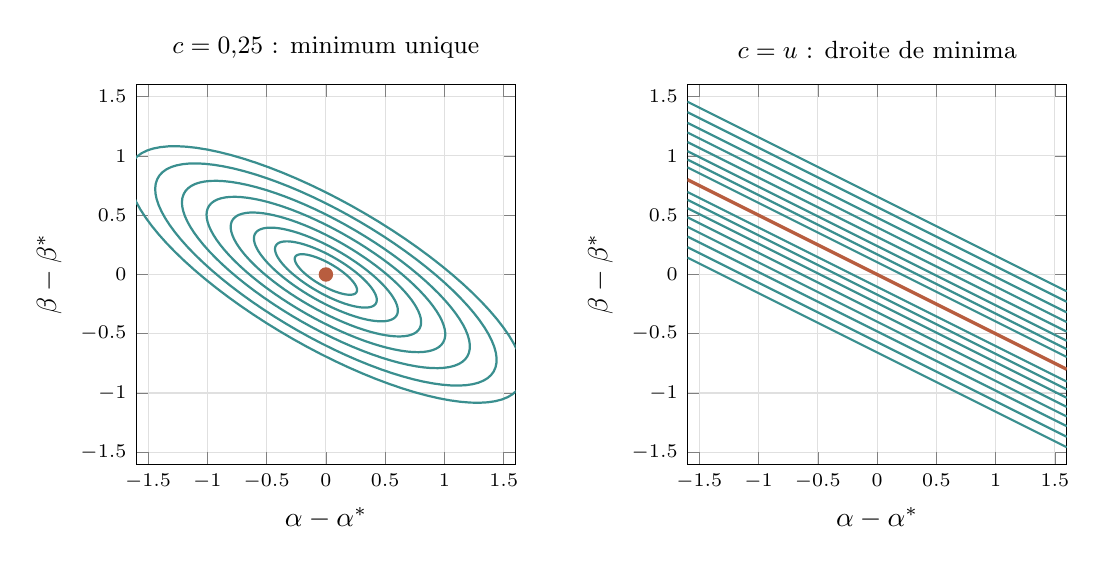
\begin{tikzpicture}
    \definecolor{oymteal}{RGB}{58,143,143}
    \definecolor{oymorange}{RGB}{184,93,63}
    \pgfplotsset{rsjs/.style={
        width=6.4cm, height=6.4cm, xmin=-1.6, xmax=1.6, ymin=-1.6, ymax=1.6,
        xtick={-1.5,-1,-0.5,0,0.5,1,1.5}, ytick={-1.5,-1,-0.5,0,0.5,1,1.5},
        xticklabel style={font=\scriptsize}, yticklabel style={font=\scriptsize},
        grid=major, grid style={black!12}, axis equal image, clip=true,
        xlabel={$\alpha-\alpha^*$}, ylabel={$\beta-\beta^*$}, title style={font=\small}}}
    \begin{axis}[rsjs, title={$c=0{,}25$ : minimum unique}]
        \pgfplotsinvokeforeach{0.15,0.4,0.8,1.4,2.2,3.2,4.5,6}{
            \addplot[oymteal, thick, domain=0:360, samples=90, variable=\u]
            ({sqrt(#1/1.68369)*cos(\u)*cos(-30.02) - sqrt(#1/16.1114)*sin(\u)*sin(-30.02)},
             {sqrt(#1/1.68369)*cos(\u)*sin(-30.02) + sqrt(#1/16.1114)*sin(\u)*cos(-30.02)});
        }
        \addplot[only marks, mark=*, mark size=2.4pt, oymorange] coordinates {(0,0)};
    \end{axis}
    \begin{axis}[rsjs, xshift=7cm, title={$c=u$ : droite de minima}]
        \pgfplotsinvokeforeach{0.15,0.4,0.8,1.4,2.2,3.2,4.5,6}{
            \addplot[oymteal, thick, domain=-1.6:1.6, samples=2] {(sqrt(#1/17.3611)/0.894427 - 0.5*x)};
            \addplot[oymteal, thick, domain=-1.6:1.6, samples=2] {(-sqrt(#1/17.3611)/0.894427 - 0.5*x)};
        }
        \addplot[oymorange, very thick, domain=-1.6:1.6, samples=2] {-0.5*x};
    \end{axis}
\end{tikzpicture}
